\chapter{Computational Implementation} \label{chap:implementation}


	This chapter presents the numerical algorithms that can be employed in computing thermodynamic equilibria. While most of these algorithms embody the concepts previously presented in the open literature, there remains a scope for improving the efficiency and capabilities of some of these algorithms through careful implementation and/or building upon them. This chapter discusses the computational implementation of the proposed thermodynamic equilibrium solver, the top-level architecture of which has been outlined in figure~\ref{fig:structure}. The program essentially consists of a parsing and input module to read the required thermodynamic data and system information followed by initialisation routines which provide the initial assemblage to a non-linear GEM routine. The assemblage from the non-linear solver is then checked to ensure global minimum is achieved at which stage the outputs are produced.
	\begin{figure}[htbp]
	 	\centering
	   	\includegraphics[width=0.65\textwidth]{figures/YJ_structure.pdf}
	   	\caption{Top-level architecture of the proposed thermodynamic equilibrium code.}
	   	\label{fig:structure}
	\end{figure}

\section{Opportunities for Novel Contributions}
Before delving into the details of a thermodynamic solver, a number of opportunities for novel contributions are presented here. The first and the foremost is integration of the thermodynamic solver within multiphysics framework \texttt{MOOSE}. \texttt{MOOSE} based applications currently leverage the thermochemistry library \texttt{Thermochimica} to perform thermodynamic equilibrium calculations. However, since \texttt{Thermochimica} was developed in FORTRAN and wasn't developed within the \texttt{MOOSE} framework, coupling it requires writing wrapper classes for every intended application. Not only does this lead to waste of time and resources, it also needs a lot of effort to maintain reliability and achieve desired performance. The new thermodynamic sover will be built within the \texttt{MOOSE} framework and will eliminate the need to write multiple wrapper classes. Furthermore, since it will use the same software quality assurance practices as \texttt{MOOSE}, it will be able to meet the desired performance standards.

	In addition to coupling, the development of the new thermodynamic code will try to achieve performance gain through advanced algorithm development. While the GEM method has little scope of improvement in itself, the performance of thermodynamic equilibrium codes can be significantly improved by improving the initialisation routines and focussing on strategies for updating the estimated phase assemblage. The strategies to achieve this goal have been presented in the following sections. Novel contributions can also be made towards global optimisation routines for thermodynamic equilibrium solvers. As shown in section~\ref{sec:opt_theory}, ensuring that a global minimum of Gibbs energy has been achieved is a challenging task and the global optimisation methods available in the literature have mostly been problem specific. Since a thermodynamic equilibrium solver needs to perform well for different kinds of problems, significant contributions can be made by implementing robust global optimisation algorithms. These strategies are discussed in the following sections.

\section{Parsing and Input}
	Calculation of thermodynamic equilibrium requires a thermodynamic database, which includes Gibbs energy expressions of the different phases and species that can exist in the system. These thermodynamic databases are developed using the well established CALculation of PHAse Diagrams (CALPHAD) method \cite{liu_wang_2016} and are available in different formats, the most commonly used being ThermoCalc (*.tdb) and ChemSage (*.dat) data file formats, which are generated by the commercial software ThermoCalc and FactSage, respectively. An example of a typical ChemSage data file is shown in figure~\ref{fig:datfile} and consists of a header block followed by information blocks for every possible phase in the system.
	\begin{figure}[htbp]
	 	\centering
	   	\includegraphics[width=\textwidth]{figures/NiKF.pdf}
	   	\caption{A marked-up example of a ChemSage data file of the \ce{Ni-K-F} system \cite{OcadizFlores18}}
	   	\label{fig:datfile}
	\end{figure}

	The data file parser for the thermodynamic equilibrium part of \texttt{Yellowjacket} has been developed in C++ and it performs the extraction of free energy expressions from *.dat thermodynamic database files (ChemSage format) and exports a list of free energy terms for each phase (or a user specified subset of phases). The data-file parser has the following capabilities:
\begin{itemize}
\itemsep-0.5em
    \item Extract system information from *.dat files and ensure that the data is consistent with the inputs and appropriate for consideration.
    \item Extract Gibbs energy terms for different phases and all the species within each phase.
    \item Store the Gibbs energy terms to ensure that terms corresponding to each phase can be selectively and conveniently retrieved.
\end{itemize}

	Another requirement for Gibbs energy minimisation is physical parameters of the system, namely, the temperature, pressure and composition. Within a multiphysics framework, these informations are required for each finite element at every time-step. In the context of the proposed Gibbs energy minimiser, the system inputs are provided by \texttt{MOOSE} which passes the information at the time the Gibbs energy minimiser is called. For standalone applications, this information can be provided as an input through the \texttt{MOOSE} input file.

\section{Initialisation}
	Much like any other optimisation problem, the choice of initial estimate plays a critical role in reducing the amount of computational time required for the solution to converge to a minimum. This need for providing initial estimates of the number of moles of phases and the mole fractions of the species in those phases creates a significant challenge. Many early softwares  created for the purpose of estimating thermodynamic equilibrium, for example SOLGASMIX, required the user to input an initial estimate. Providing such initial estimates relied on the intuition of the user and was often very inconvenient for the user, especially when working with complex systems and/or systems where finding estimates from intuition was not straightforward.
%	, it also left the door open to encountering an initial assemblage far from the actual, thus resulting in large computational costs.
	To overcome the need for the user to enter the initial estimates,  Eriksson and Thompson \cite{Eriksson89} proposed an initialisation algorithm called \textit{levelling} that has found widespread application in thermodynamic equilibrium softwares. Subsequently, Piro and Simunovic \cite{Piro12a} proposed the \textit{post-levelling} method as an extension to levelling in order to further improve the initial estimate.

	\subsection{Linear solver}
	The levelling algorithm was developed to accelerate the rate of convergence by eliminating the phases and species that have an insignificant contribution in the final phase assemblage. The algorithm is based on a temporary treatment of all species and phases in the system as pure stoichiometric phases. Mathematically, this amounts to temporarily converting the non-linear optimisation problem into a linear optimisation problem and the algorithm for the computational implementation has been illustrated in figure~\ref{fig:levelling}.
	\begin{figure}[htb]
		\centering
		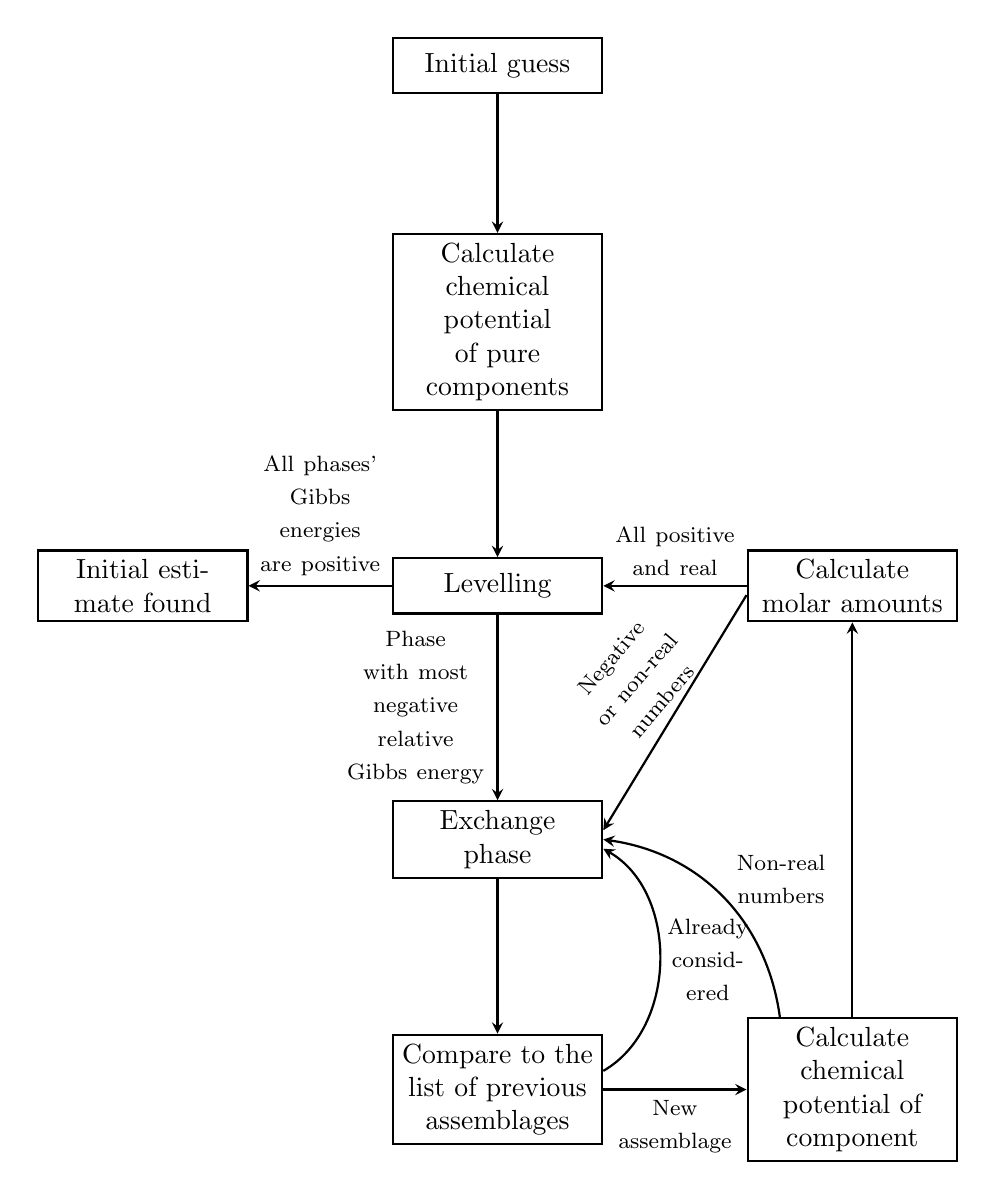
\begin{tikzpicture}[auto,
    			block_center/.style ={rectangle, draw=black, thick, fill=white, text width=0.2\textwidth, text centered, minimum height=2em},
    			block_side/.style ={rectangle, draw=black, thick, fill=white, text width=0.2\textwidth, text centered, minimum height=2em},
			block_noborder/.style ={rectangle, draw=none, thick, fill=none, text width=0.15\textwidth, text centered, minimum height=0.5em},
			block_small/.style ={rectangle, draw=none, thick, fill=none, text width=0.1\textwidth, text centered, minimum height=0.5em},
			line/.style ={draw, thick, -stealth}]
    			% Outlining the flowchart using the PGF/TikZ matrix funtion
    			\matrix [column sep=0.15\textwidth,row sep=5em] {
      				{} & \node [block_center] (01) {Initial guess}; & {}\\
      				{} & \node [block_center] (11) {Calculate chemical potential of pure components}; & {}\\
      				\node [block_side] (20) {Initial estimate found}; & \node [block_center] (21) {Levelling}; & \node [block_side] (22) {Calculate molar amounts};\\
      				{} & \node [block_center,yshift=-1cm] (31) {Exchange phase}; & {}\\
      				{} & \node [block_center] (41) {Compare to the list of previous assemblages}; & \node [block_side] (42) {Calculate chemical potential of component};\\
    			};	% end matrix
    			% connecting nodes with paths
    			\begin{scope}[every path/.style=line]
      				\path (01) edge (11);
     				\path (11) edge (21);
      				\path (21) edge node[block_noborder,anchor=east]{\footnotesize{Phase with most negative relative Gibbs energy}} (31);
      				\path (31) edge (41);
      				\path (22) edge node[block_noborder,anchor=south]{\footnotesize{All positive and real}} (21);
      				\path (21) edge node[block_noborder,anchor=south]{\footnotesize{All phases' Gibbs energies are positive}} (20);
      				\path (41) edge node[block_noborder,anchor=north]{\footnotesize{New assemblage}} (42);
      				\path (42) edge (22);
      				\path[-] (22.185) edge node[block_noborder,rotate=49.5,anchor=south]{\footnotesize{Negative or non-real numbers}} (31.5);
      				\path[-] (41.10) edge[bend right=60] node[block_small,anchor=west,shift={(-0.125cm,0)}]{\footnotesize{Already considered}} (31.355);
     				\path[-] (42.135) edge[bend right=37] node[block_small,anchor=west,shift={(0,0.225cm)}]{\footnotesize{Non-real numbers}} (31.360);
    			\end{scope}
 		\end{tikzpicture}
  		\caption{Illustration of the levelling algorithm \cite{Loukusa:2014aa}}
  		\label{fig:levelling}
 	\end{figure}

	Since the Gibbs energy is a relative thermodynamic function and the Gibbs energies of each component element are not related to one another \cite{Eriksson89}, it is possible to numerically alter the Gibbs energy of each phase while preserving the elemental differences. Levelling is performed by representing the set of Gibbs energies relative to the collection of phases assumed to be most stable and uses a relative Gibbs energy function called the \textit{absolute Gibbs energy} by Eriksson and Thompson and is the Gibbs energy of the pure species per atom in the species as shown in equation~\eqref{eq:absGibbs}
	\begin{equation}\label{eq:absGibbs}
		\hat{G}_i = \frac{G_j}{\sum_{j=1}^C \nu_{ij}}
	\end{equation}

	The levelling process determines the combination of phases yielding the lowest Gibbs energy by evaluating a combination of Gibbs energies on a relative basis. A phase that has a negative relative Gibbs energy with respect to the assemblage indicates that a phase in the assemblage must be replaced by the current phase to achieve a lower integral Gibbs energy.

	Mathematically, levelling is achieved through an iterative process that systematically adjusts fixed combinations of phases, subject to the linear equality and inequality mass balance constraints, to progressively minimise the GIbbs energy of the system \cite{Piro12a}. At iteration $m+1$, the adjustment to be applied to the relative Gibbs energy of phase $i$ is defined by \cite{Eriksson89}:
	\begin{equation} \label{eq:lev_adj}
		\begin{aligned}
			d \hat{G}_i^{m\rightarrow m+1} &= \sum_{j=1}^{C} c_{i,j} d \Gamma_j^{m\rightarrow m+1}\\
			\hat{G}_i^{m+1} &= \hat{G}_i^{m} - d \hat{G}_i^{m\rightarrow m+1}
		\end{aligned}
	\end{equation}
	where, $c_{i,j}$ denotes the atomic fraction of element $j$ in species $i$ and $d \Gamma_j^{m\rightarrow m+1}$ is the adjustment applied to the chemical potential of element $j$, which in turn is determined by the most stable phases found at iteration $m$.

	In  matrix form, the overall mass balance constraint can be represented as \cite{Piro12a}
	\begin{equation} \label{eq:levMB_mat}
		\mathbf{A^T} \mathbf{n}= \mathbf{b}
	\end{equation}
	where $\mathbf{A} \in \mathbb{R}^{E \times \Phi}$ represents the stoichiometric matrix, $\mathbf{n} \in \mathbb{R}^{\Phi }$ denotes the column vector of the number of moles of each phase, and $\mathbf{b} \in \mathbb{R}^{E}$ is the column vector with the total mass of each element in the system. When equation~\ref{eq:levMB_mat} is used in levelling, $\Phi = E$.

	The initial guess for the levelling method is the most chemically stable form of each element and the stoichiometric matrix $\mathbf{A^T}$ in equation~\eqref{eq:levMB_mat} becomes a diagonal matrix. Subsequently, provided all elements of vector $\mathbf{b}$ are positive, all the elements of $\mathbf{n}$ must also be positive. However, the diagonality of the stoichiometric matrix is not preserved over subsequent iteration and it assumes a non-symmetric sparse form. In fact, the matrix $\mathbf{A^T}$ might become rank deficient if proper care is not taken while selecting the phase assemblage.

	In levelling, since the number of phases in the system is equal to the number of elements, the element potentials can then be uniquely determined from the current estimated phase assemblage by solving the following system of linear equations:
	\begin{equation} \label{eq:levEP_mat}
		\mathbf{A^T} \boldsymbol{\Gamma} = \boldsymbol{\mu}
	\end{equation}
	where $\boldsymbol{\Gamma} \in \mathbb{R}^{E} $ and $\boldsymbol{\mu} \in \mathbb{R}^{\Phi}$.

	The next step in levelling is updating the phase assemblage in accordance with equation~\eqref{eq:lev_adj}. A  species with a positive $\hat{G}_i^{m+1}$ would yield a thermodynamically less stable assemblage and is left out along with phases with insignificant contributions to final equilibrium while the phase with the most negative $\hat{G}_i^{m+1}$ is introduced into the assemblage by replacing a phase in the previous assemblage. The phase assemblage at this stage must meet three requirements. First, the number of moles of all phase in $\mathbf{n}$ must be non-negative and real. Second, all the elements of the vector $\boldsymbol{\Gamma}$ must be real. Finally, the phase assemblage must not have been previously considered. If the phase assemblage does not meet any of these requirements, the phase with the second lowest relative Gibbs energy must be considered, and so on.

	While the criteria for the phase to be added in the system was well established by Eriksson and Thompson, a criterion to select the phase to be replaced wasn't proposed and, typically, local iterations were performed to systematically traverse through the candidate phases until a particular combination yielded an entire set of non-negative and real mole numbers \cite{Eriksson89}. The number of these local iterations rapidly grows with the number of elements in the system and an alternative named \emph{Euclidean norm} was proposed by Piro and Simunovic \cite{Piro12a}. This method has been described in sec.~\ref{sec:Euclidean}

	Once the new phase has been exchanged with one of the existing phases and its acceptability has been determined, levelling step is repeated until no phases with negative absolute Gibbs energy remain in the system. At this stage, the assemblage can be passed on to a non-linear solver as the initial estimate.


	\begin{figure}[htbp]
		\centering
		\includegraphics[width=\textwidth]{figures/Levelling_illustration}
		\caption{Illustration of the levelling process for a binary system of \ce{U-O} at each iteration (1 \si{\mole} \ce{U}, 2.2 \si{\mole} \ce{O}, 298.15 \si{\kelvin}, 1 \si{atm}) \cite{Piro11b}.}
		\label{fig:lev_illus}
	\end{figure}

	An example of the levelling method is presented in figure~\ref{fig:lev_illus}. In the illustration, in the first iteration, the phase with the most negative Gibbs energy is paired with another phase that together has non-negative molar quantities. At the end of iteration 0, choosing solid \ce{UO2} as the phase with the most negative relative Gibbs energy and arbitrarily choosing solid \ce{UO3} to pair it with, the equivalent Gibbs energies of pure uranium and pure oxygen are computed and followed by the element potentials $\Gamma_{\ce{U}}$ and $\Gamma_{\ce{O}}$ (represented by the dashed red line). The levelling procedure is then applied and the relative Gibbs energies of the terms are calculated.

	At the start of iteration 1, the relative Gibbs energy of solid \ce{U3O8} is negative with respect to the combination of solid \ce{UO2} and solid \ce{UO3}, indicating it must be introduced in the assemblage. The internal linear solver then determines the phase that must be replaced and the iterative process continues with the updated phase assemblage.

	At the end of the levelling procedure, the assemblage has the lowest Gibbs energy with all other phases being positive with respect to the assemblage. The Gibbs energy of the pure stoichiometric system is thereby minimised. For the example presented in figure~\ref{fig:lev_illus}, the levelling solver converges in only 3 iterations. According to Eriksson and Thompson \cite{Eriksson89}, the computational expense using levelling can be up to two to five times lower than the general equilibrium calculations.

	Mathematically, the levelling  process always respects the Gibbs phase rule, mass balance and the Gibbs' criterion and the number of iterations required to achieve convergence is typically close to the number of elements. This results in significant computational advantage when considering exceeding large number of possible phase combinations as the number of elements in the system grow making levelling an excellent choice as an initialisation routine.

	\subsection{Post-levelling}
	Developed by Piro and Simunovic \cite{Piro12a}, the post-levelling method is an extension to the levelling method and can be used to refine the assemblage provided by the levelling method by accounting for the ideal mixing of the phases and relaxing the assumption that the phases are pure. Thus, post-levelling acts as an intermediate step between levelling and the non-linear solver. While post-levelling resembles the non-linear solver in the incorporation of compositional component in the chemical potential of the solution phase constituents, the primary distinction between them is that post-levelling considers only dominant phases identified by levelling as compared to the non-linear solver which considers all the constituents. Furthermore, the non-linear solver also considers non-ideal behaviour.

		The chemical potential term in post-levelling takes the following form:
		\begin{equation}
			\begin{aligned}
				\mu_{i(\lambda} &= g_{i(\lambda)}^0 + RT \ln{(x_{i(\lambda)})} \\
				x_{i(\lambda)} &= \frac{n_{i(\lambda)}}{\sum_{k=1}^{N_{\lambda}}n_{k(\lambda)}}
			\end{aligned}
		\end{equation}
		where $N_{\lambda}$ is the number of constituents in solution phase $\lambda$ identified by levelling and is less than the actual constituents in the phase. The element potentials can then be computed using equation~\eqref{eq:levEP_mat} and an iterative process similar to levelling can be followed.

		A demonstration of the post-levelling method in predicting the element potentials of combustion products from a coal fire shows that compared to levelling, post levelling calculations provide values much closer to the equilibrium values. As a result, the rate of convergence of the non-linear solver improves by a large factor.  While exact gains depend on the non-linear solver, line-search algorithm and the strategy for updating the estimated phase assemblage, relative performance gains can be easily envisaged even though post-levelling process incurs additional computational cost. This can be attributed to the fact that the cost of post-levelling is negligible in comparison to the cost of a single iteration in a non-linear solver \cite{Piro12a}.

	\subsection{Euclidean norm} \label{sec:Euclidean}
	The Euclidean norm method was proposed by Piro and Simunovic \cite{Piro12a}, to strategically rank the best candidate phases to accommodate a new phase change. The Gibbs phase rule requires that when the thermodynamic degree of freedom $F$ equals zero, a phase must be removed in order to introduce a new phase. Determining whether a candidate phase is feasible is the most expensive task within the global iteration cycles as it requires solution of a simultaneous equation to ensure that the Hessian matrix is non-singular \cite{Piro12a}. If there are multiple candidate phases, this iterative process must be repeated for each candidate.

	The Euclidean norm method systematically ranks the best candidates to be withdrawn from the system without having to perform an exhaustive search. The method is based on the principle that the best candidate phase to be withdrawn from the current assemblage has the most similar atomic composition to the phase that has to be added to the system.

	The atomic fraction of element $j$ in a pure stoichiometric phase $\omega$ is represented as:
	\begin{equation}
		c_{\omega,j} = \frac{c_{\omega,j}}{\sum_{k=1}^{E} x_{i(\omega)}\nu_{\omega,j}}
	\end{equation}

	Similarly, in the solution phase  $\lambda$, the atomic fraction of element $j$ is computed by
	\begin{equation}
		c_{\lambda,j} = \frac{\sum_{i=1}^{N_{\lambda}} \nu_{i,j}}{\sum_{i=1}^{N_{\lambda}} \sum_{k=1}^{E} x_{i(\lambda) \nu_{i,k}}}
	\end{equation}

	Denoting the atom fraction of the element $j$ in the new phase that is to be introduced into the system with $c_{\phi,j}^{*}$, the difference between this phase and the phases currently in the assemblage is given by the Euclidean norm of each phase $\phi$
	\begin{equation}
		\|c_\phi\|_2 = \sqrt{\sum_{j=1}^{E} \left(c_{\phi,j} - c_{\phi,j}^{*}\right)^2}
	\end{equation}

	The phase with the lowest Euclidean norm has the most similar composition to the phase to be introduced in the assemblage. In case the resulting assemblage does not meet the criterion to be a valid assemblage, the phase with the second lowest Euclidean norm can be introduced and so on.

	As shown in figure~\ref{fig:PEA_gains}, the overall computational expense of thermodynamic calculations is significantly reduced when post-levelling and Euclidean norm methods are utilised \cite{Piro12a}. These performance gains can offer a significant advantage when considering multiphysics simulations where thermodynamic equilibrium is often the most computationally expensive calculation.

	\begin{figure}[htbp]
		\centering
		\includegraphics[width=0.65\textwidth]{figures/PEA_Gains}
		\caption{Performance gains when employing post-levelling and Euclidean-norm algorithms \cite{Piro12a}.}
		\label{fig:PEA_gains}
	\end{figure}


	\subsection{Temporal series estimate}
	While in most cases levelling and post-levelling methods can provide initial assemblages close to the final assemblage, using the assemblage from a previous time step in multiphysics codes can often provide much closer estimates to the final assemblage. In time-dependent multiphysics simulations, this can result in significant performance gains as has been recently shown through the implementation of this strategy in \texttt{Thermochimica} \cite{Poschmann:2019aa}. These performance gains can be attributed to the fact that the convergence of the non-linear solver can be significantly accelerated by providing initial estimates close enough to the final assemblage. This temporal initialisation strategy has been illustrated in figure~\ref{fig:temp_init}
	\begin{figure}
		\centering
		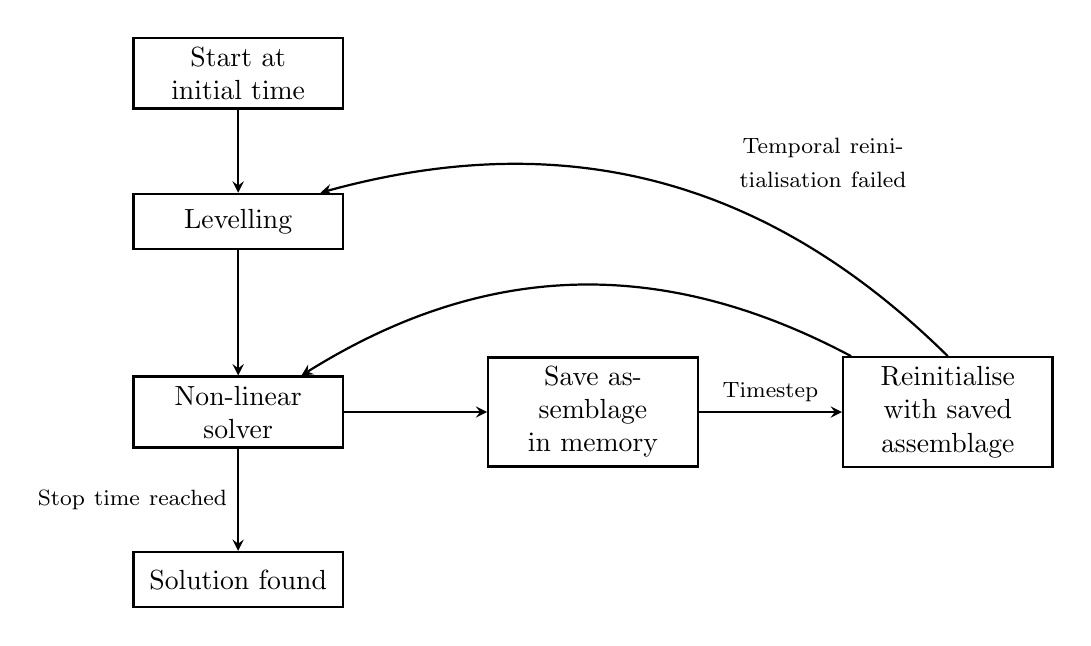
\begin{tikzpicture}[auto,
    			block_center/.style ={rectangle, draw=black, thick, fill=white, text width=0.2\textwidth, text centered, minimum height=2em},
    			block_side/.style ={rectangle, draw=black, thick, fill=white, text width=0.2\textwidth, text centered, minimum height=2em},
			block_noborder/.style ={rectangle, draw=none, thick, fill=none, text width=0.2\textwidth, text centered, minimum height=0.5em},
			block_small/.style ={rectangle, draw=none, thick, fill=none, text width=0.1\textwidth, text centered, minimum height=0.5em},
			line/.style ={draw, thick, -stealth}]
    			% Outlining the flowchart using the PGF/TikZ matrix funtion
    			\matrix [column sep=0.15\textwidth,row sep=3em] {
      				\node [block_center] (00) {Start at initial time}; & {} & {}\\
      				\node [block_center] (10) {Levelling}; & {} & {}\\
				\node [block_center,yshift=-1cm] (20) {Non-linear solver}; &  \node [block_side,yshift=-1cm] (21) {Save assemblage in memory}; & \node [block_side,yshift=-1cm] (22) {Reinitialise with saved assemblage};\\
      				\node [block_side] (30) {Solution found}; & {} & {}\\
    			};	% end matrix
    			% connecting nodes with paths
    			\begin{scope}[every path/.style=line]
      				\path (00) edge (10);
     				\path (10) edge (20);
      				\path (20) edge node[block_noborder,anchor=east]{\footnotesize{Stop time reached}} (30);
      				\path (20) edge (21);
      				\path (21) edge node[block_noborder,anchor=south]{\footnotesize{Timestep}} (22);
      				\path[-] (22.90) edge[bend right] node[block_noborder,anchor=west,shift={(0.75cm,0.25cm)}]{\footnotesize{Temporal reinitialisation failed}} (10);
      				\path[-] (22) edge[bend right] (20);
    			\end{scope}
 		\end{tikzpicture}
  		\caption{Illustration of the temporal series initialisation algorithm.}
  		\label{fig:temp_init}
 	\end{figure}

	The details of the implementation of the temporal initialisation strategy in \texttt{Yellowjacket} have not yet been set in stone but, based on \texttt{Thermochimica} acceleration results obtained by Poschmann et al. \cite{Poschmann:2019aa} , a significant performance gain is foreseen which justifies the use of this strategy especially in coupled multiphysics problems where thermodynamic equilibrium calculations are impediment to significant performance gains. However, this might also lead to a drastic increase in memory requirement and a compromise must be made between  computing time gains and increased memory requirements.

	\subsection{Boundary value estimate}
	For the case where Gibbs energy minimisation is performed on a 2D/3D mesh, very good initial estimates can conceivably be provided to the non-linear solver by exploiting the results from the neighbouring solutions in space at the same time step. As an example, the final assemblage of element A on the finite element mesh shown in figure~\ref{fig:BV_Illustration} can be used as the initial assemblage for element B. This initialisation scheme relies on the principles of continuum between adjacent cells, i.e., if the mesh is sufficiently resolved, the difference between system potentials (temperature, pressure and chemical potentials) between two neighbouring cells must be small.
	\begin{figure}[htbp]
		\centering
		\includegraphics[width=0.35\textwidth]{figures/BV_FEM}
		\caption{Illustration of the boundary value initialisation on a finite element mesh \cite{Piro17}.}
		\label{fig:BV_Illustration}
	\end{figure}

	While this approach is well suited to simulations on finite element meshes and reduces the need to re-evaluate the estimated assemblage of stable phases, it might lead to a less than optimal estimate for elements close to a moving interface (for example, close to a melting boundary). Also, this approach does not lend itself well to parallel computing using MPI and thus might actually be ineffective for large problems where MPI can significantly speed up calculations. However, the approach is a potential avenue that can be explored but is not the primary focus.

\section{Non-linear solver}
	The linear solver can often provide estimates close to the final assemblage of the system and in certain circumstances, such as for systems with only pure 	stoichiometric species, it might be able to predict the equilibrium assemblage. However, almost always, further computations are required to arrive at the final assemblage especially in cases where the phases have more than one species with significant contribution to the Gibbs energy. This situation arises more often than not and a non-linear solver is required to handle the non-linearities arising from the logarithmic term in the compositional component of the chemical potentials.

	For the sake of completeness of the argument, the conditions for equilibrium are restated below:
	\begin{enumerate}
		\item The mass balance constraint must be satisfied.
		\item The Gibbs' phase rule must be satisfied.
		\item The integral Gibbs energy must be at a global minimum.
	\end{enumerate}

	The following subsidiary conditions arise from the constraints
	\begin{enumerate}[label=\Alph*.]
		\item The number of moles of any species must be positive.
		\item The sum of mole fractions must be one (inherent in the Gibbs energy method).
	\end{enumerate}

	The GEM method presented by White \textit{et al.} \cite{White:58} can constrain conditions 1 and 2 while optimising condition 3.  The subsidiary condition B is inherent in the method and is always satisfied but care must be taken to ensure that subsidiary condition A is met. However, in most cases, condition 1 is not initially satisfied and GEM optimises conditions 1 and 3 simultaneously \cite{Eriksson71}. The derivation of the GEM method is  given below \cite{Piro11b}.

	The quantity to be minimised,  the integral Gibbs energy of the system, depends on the molar amounts $n_i$ of the species in the system, which are subject to the mass balance constraints given by the individual components in the system. In dimensionless form, the Gibbs energy can be represented as:
	\begin{equation}
		G^m = \sum_{\lambda=1}^{\Lambda} \left(\frac{\mu_{i(\lambda)}^m}{RT}\right)n_{i(\lambda)}^m + \sum_{\omega=1}^{\Omega}\left(\frac{\mu_{\omega}^m}{RT}\right)n_{i(\omega)}^m
	\end{equation}
	where, the variable $G^m$ represents the Gibbs energy at iteration $m$ and is expressed in the dimensionless form as by doing so we can avoid the division by $RT$ at every iteration step, thus increasing efficiency. It must be noted that the chemical potential of the stoichiometric phase, ${\mu_{i(\omega)}^m}$, is by definition fixed but the superscript has been retained for the uniformity of notation.  The mass balance for component $j$ is given as:
	\begin{equation}
		b_j^m = \sum_{\lambda=1}^{\Lambda} n_{i(\lambda)}^m \nu_{i,j} + \sum_{\omega=1}^{\Omega}n_{\omega}^m \nu_{\omega ,j}
	\end{equation}
	where $b_j^m$ is the estimated molar quantity and not the true mass of element $j$ in the system \cite{Piro11b}. The mass constraint (condition A) requires that
	\begin{equation}
		b_j - b_j^m = 0
	\end{equation}
	To arrive at the quadratic approximation of the Gibbs energy function, a Taylor expansion is performed:
	\begin{equation}
		\begin{aligned}
		Q^{m+1} = G^m &+ \left. \sum_{\omega=1}^{\Omega} \delta_{\omega} \frac{\partial G^m}{\partial n_{\omega}^m}\right\vert_{n_{\omega}^m = n_{\omega}^{m+1}} \\
				&+ \left. \sum_{\lambda=1}^{\Lambda} \delta_{i} \frac{\partial G^m}{\partial n_{i(\lambda)}^m}\right\vert_{n_{i(\lambda)}^m = n_{i(\lambda)}^{m+1}} \\
				&+ \frac{1}{2} \left. \sum_{\omega=1}^{\Omega} \delta_{\omega}^2 \frac{\partial^2 G^m}{\partial \left(n_{\omega}^m\right)^2}\right\vert_{n_{\omega}^m = n_{\omega}^{m+1}} \\
				&+ \frac{1}{2} \left. \sum_{\lambda=1}^{\Lambda} \sum_{i=1}^{N_{\lambda}} \sum_{l=1}^{N_{\lambda}} \delta_{i} \delta_{l} \frac{\partial^2 G^m}{\partial n_{i(\lambda)}^{m} \partial n_{l(\lambda)}^{m}} \right\vert_{n_{i(\lambda)}^m = n_{i(\lambda)}^{m+1}}
		\end{aligned}
	\end{equation}
	where $\delta_i  = n_{i(\lambda)}^{m+1} - n_{i(\lambda)}^m$ and $\delta_{\omega}  = n_{\omega}^{m+1} - n_{\omega}^m$. By the definition of chemical potential, the first order derivatives take the following form:
	\begin{gather}
		\frac{\partial G^m}{\partial n_{i(\lambda)}^{m}} = \frac{\mu_{i(\lambda)}^{m}}{RT} \\
		\frac{\partial G^{\omega}}{\partial n_{\omega}^{m}} = \frac{\mu_{\omega}^{m}}{RT}
	\end{gather}
	and the second order derivatives can be represented as:
	\begin{gather}
		\frac{\partial^2 G^m}{\partial \left(n_{i(\lambda)}^{m}\right)^2} = \frac{1}{n_{i(\lambda)}^{m}} - \frac{1}{n_{\lambda}^{m}}\\
		\left. \frac{\partial^2 G^m}{\partial n_{i(\lambda)}^{m} \partial n_{l(\lambda)}^{m}}\right\vert_{l\neq i} =  - \frac{1}{n_{\lambda}^{m}} \\
		\frac{\partial^2 G^m}{\partial \left(n_{\omega}^{m}\right)^2} = 0
	\end{gather}

	Substituting these expressions into the Taylor expansion results in the following:
	\begin{equation}\label{eq:Taylor_Obj}
		\begin{aligned}
		Q^{m+1} = G^m &+  \sum_{\omega=1}^{\Omega} \delta_{\omega} \frac{\mu_{\omega}^{m}}{RT}\\
				&+ \sum_{\lambda=1}^{\Lambda} \delta_{i} \frac{\mu_{i(\lambda)}^m}{RT}\\
				&+ \frac{1}{2} \sum_{\lambda=1}^{\Lambda} \sum_{i=1}^{N_{\lambda}} n_{i(\lambda)}^{m} \left(\frac{\delta_i}{n_{i(\lambda)}^{m}} - \frac{\delta_{\lambda}}{n_{\lambda}^{m}} \right)^2
		\end{aligned}
	\end{equation}
	where, $\delta_{\lambda} = n_{\lambda}^{m+1} - n_{\lambda}^m$

	 To find the next approximation to the desired solution, we can minimise $Q^{m+1}$ subject to the mass balance constraint and restricting $n$ to positive values \cite{White:58}. The constrained optimisation problem can be solved using the Lagrange method of undetermined multipliers \cite{Nocedal06} where the Lagrangian function in terms of the objective function and the constraints is written as follows:
	 \begin{equation}
	 	L = Q^{m+1} + \sum_{E}^{j=1} \pi_{m+1}^{j}\left( b_j - b_j^{m}\right)
	 \end{equation}
	 where the undetermined Lagrange multipliers are denoted by $\pi_{m+1}^{j}$. This formulation allows for the mass balances to be corrected when the initial estimates of mole numbers do not satisfy the mass balance constraints thereby helping in simultaneously minimising the Gibbs energy of the system and residuals of the mass constraints \cite{Piro11b}. The minimum of the Lagrangian can be found by finding the points where the partial derivatives of the Lagrangian with respect to the molar amounts and the Lagrange multiplier are zero. This results in the following system of equations:
	 \begin{gather}
			\frac{\partial L}{\partial n_{i(\lambda)}^{m}} = \frac{\mu_{i(\lambda)}^{m}}{RT} - \sum_{j=1}^{E} \nu_{i,j} \pi_j^{m+1} + \left(\frac{n_{i(\lambda)}^{m+1}}{n_{i(\lambda)}^{m}} - \frac{n_{\lambda}^{m+1}}{n_{\lambda}^{m}}\right) = 0\\
			\frac{\partial L}{\partial n_{\omega}^{m}} = \frac{\mu_{\omega}^{m}}{RT} - \sum_{j=1}^{E} \nu_{\omega,j}\pi_{m+1}^{j} = 0
	\end{gather}
	Rearranging and solving the above equation gives:
	\begin{equation}
			n_{i(\lambda)}^{m+1} = n_{i(\lambda)}^{m} \left( -\frac{\mu_{i(\lambda)}^{m}}{RT} +  \frac{n_{\lambda}^{m+1}}{n_{\lambda}^{m}} + \sum_{j=1}^{E} \nu_{i,j} \pi_j^{m+1} \right)
	\end{equation}
	 and using the mass balance:
	 \begin{equation}
			b_j = \sum_{\lambda=1}^{\Lambda} \sum_{i=1}^{N_\lambda} \left( -\frac{\mu_{i(\lambda)}^{m}}{RT} +  \frac{n_{\lambda}^{m+1}}{n_{\lambda}^{m}} + \sum_{j=1}^{E} \nu_{i,j} \pi_j^{m+1} \right)n_{i(\lambda)}^{m} \nu_{i,j} + \sum_{\omega=1}^{\Omega}n_{\omega}^{m} \nu_{\omega,j}
	\end{equation}

	The above equation can be rearranged to arrive at the form used by Eriksson and Ros\'en \cite{Eriksson73}:
	\begin{equation}\label{eq:GEM1}
		\sum_{j=1}^{E} r_{j,k}\pi_{j}^{m+1} + \sum_{\lambda=1}^{\Lambda}\pi_{\lambda}^{m+1} \varphi_{\omega,j}^{m} + \sum_{\omega=1}^{\Omega}n_{\omega}^{m} \nu_{\omega,j}
		= b_j + \sum_{\lambda=1}^{\Lambda} \sum_{i=1}^{N_\lambda} \left( \frac{\mu_{i(\lambda)}^{m}}{RT} -1 \right)n_{i(\lambda)}^{m} \nu_{i,j}
	\end{equation}
	where, $$r_{j,k} = \sum_{\lambda=1}^{\Lambda} \sum_{i=1}^{N_\lambda} n_{i(\lambda)}^{m} \nu_{i,j}\nu_{i,k}$$ $$\varphi_{\omega,j}^{m} = \sum_{i=1}^{N_\lambda} n_{i(\lambda)}^{m} \nu_{i,j}$$ $$\pi_{\lambda}^{m+1} = \left(\frac{n_{\lambda}^{m+1}}{n_{\lambda}^{m}}\right) -1$$

	The  form of the minimisation problem in equation~\eqref{eq:GEM1} is relevant to programming since the set of the undetermined Lagrange multipliers $\pi_{j}^{m+1}$ are in fact the chemical potentials and the mass balance can be enforced using the undetermined Lagrange multipliers $\pi_{\lambda}^{m+1}$. The chemical potential of the elements can then be computed using:
	\begin{equation}\label{eq:GEM2}
		\sum_{j=1}^{E} \pi_{j}^{m+1} \varphi_{\lambda,j}^{m} = \sum_{i=1}^{N_\lambda} \left(\frac{\mu_{i(\lambda)}^{m}}{RT}\right)n_{i(\lambda)}^{m}
	\end{equation}
	 Conversely, the chemical potential of the system components can be constrained since the chemical potential of pure stoichiometric phases is fixed \cite{Piro11b}:
	 \begin{equation}\label{eq:GEM3}
		\frac{\mu_{\omega}^{m}}{RT} = \sum_{j=1}^{E} \nu_{\omega,j} \pi_{j}^{m+1}
	\end{equation}

	\subsection{Matrix representation}
	The system of $(E+\Lambda+\Omega)$ linear equations formed by equations~\eqref{eq:GEM1}, \eqref{eq:GEM2} and \eqref{eq:GEM3} contains $(E+\Lambda+\Omega)$ variables and can conveniently be represented in the matrix representation as follows:
	\begin{equation}\label{eq:GEM_mat}
		\mathbf{H}\cdot\boldsymbol{\pi} = \boldsymbol{\zeta}
	\end{equation}
	where the Hessian matrix ($\mathbf{H}$) can be written as:
	\begin{equation}\label{eq:Hessian_mat}
        \mathbf{H} =
        \begin{bmatrix}
            r_{j=1,k=1} & \dots & r_{j=1,k=C} & \phi_{j=1,\lambda=1} & \dots & \phi_{j=1,\lambda=\Lambda} & \nu_{j=1,\omega=1} & \dots & \nu_{j=1,\omega=\Omega} \\
            \vdots & \ddots & \vdots & \vdots & \ddots & \vdots & \vdots & \ddots & \vdots \\
            r_{j=C,k=1} & \dots & r_{j=C,k=C} & \phi_{j=C,\lambda=1} & \dots & \phi_{j=C,\lambda=\Lambda} & \nu_{j=C,\omega=1} & \dots & \nu_{j=C,\omega=\Omega} \\
            \phi_{\lambda=1,j=1} & \dots & \phi_{\lambda=1,j=C} & 0 & \dots & 0 & 0 & \dots & 0 \\
            \vdots & \ddots & \vdots & \vdots & \ddots & \vdots & \vdots & \ddots & \vdots \\
            \phi_{\lambda=\Lambda,j=1} & \dots & \phi_{\lambda=\Lambda,j=C} & 0 & \dots & 0 & 0 & \dots & 0 \\
            \nu_{\omega=1,j=1} & \dots & \nu_{\omega=1,j=C} & 0 & \dots & 0 & 0 & \dots & 0 \\
            \vdots & \ddots & \vdots & \vdots & \ddots & \vdots & \vdots & \ddots & \vdots \\
            \nu_{\omega=\Omega,j=1} & \dots & \nu_{\omega=\Omega,j=C} & 0 & \dots & 0 & 0 & \dots & 0
        \end{bmatrix}
    \end{equation}
    and $\boldsymbol{\pi}$ and $\boldsymbol{\zeta}$ which denote the unknown and constraint vectors respectively take the following forms:
    \begin{equation}\label{eq:LagMult_mat}
        \boldsymbol{\pi} =
        \begin{bmatrix}
            \pi_{j=1}^{m+1} \\
            \vdots \\
            \pi_{j=E}^{m+1} \\
            \pi_{\lambda=1}^{m+1} \\
            \vdots \\
            \pi_{\lambda=\Lambda}^{m+1} \\
            \pi_{\omega=1}^{m+1} \\
            \vdots\\
            \pi_{\omega=\Omega}^{m+1}
        \end{bmatrix}
    \end{equation}

     \begin{equation}\label{eq:Constraint_mat}
        \boldsymbol{\zeta} =
        \begin{bmatrix}
            b_{j=1} +  \sum_{\lambda=1}^{\Lambda} \sum_{i=1}^{N_\lambda} \left( \frac{\mu_{i(\lambda)}^{m}}{RT} -1 \right)n_{i(\lambda)}^{m} \nu_{i,j=1}\\
            \vdots \\
            b_{j=E} +  \sum_{\lambda=1}^{\Lambda} \sum_{i=1}^{N_\lambda} \left( \frac{\mu_{i(\lambda)}^{m}}{RT} -1 \right)n_{i(\lambda)}^{m} \nu_{i,j=E}\\
            \sum_{i=1}^{N_{\lambda=1}} \left( \frac{\mu_{i(\lambda=1)}^{m}}{RT} -1 \right)n_{i(\lambda=1)}^{m} \\
            \vdots \\
            \sum_{i=1}^{N_{\lambda=\Lambda}} \left( \frac{\mu_{i(\lambda=\Lambda)}^{m}}{RT} -1 \right)n_{i(\lambda=\Lambda)}^{m} \\
            \frac{\mu_{\omega=1}^{m}}{RT} \\
            \vdots\\
            \frac{\mu_{\omega=\Omega}^{m}}{RT} \\
        \end{bmatrix}
    \end{equation}

The unknown column vector $\boldsymbol{\pi}$ is computed through a linear equation solver and used to update the molar quantities of each species and phase at each  iteration. The matrix $\mathbf{H}$ being a Hessian is necessarily square and symmetric and solving equation~\eqref{eq:GEM_mat} can be viewed as solving the Karush-Kahn-Tucker (KKT) optimality condition via Newton's method \cite{Nocedal06}.
	\subsection{Numerical implementation}
	The system of non-linear equations can be solved using either the Newton-Raphson method. Newton-Raphson method depends on solving  equation~\eqref{eq:GEM_mat} and is an $\mathcal{O}(N^3)$ operation.
	An integral component of the solver is an appropriate line-search algorithm to determine how far the system should progress along the direction vectors. The functional norm of the Lagrangian is an effective choice to ensure convergence and is defined as \cite{Piro17}:
	\begin{equation}
	\begin{aligned}
		\|f\|^2 = &\sum_{j=1}^{C}\left(\sum_{\lambda=1}^{\Lambda} n_\lambda \sum_{i=1}^{N_\lambda} x_{i(\lambda)}\nu_{i,j} + \sum_{\omega=1}^{\Omega}n_{\omega}\nu_{\omega,j} - b_j\right)^2 \\
		&+ \sum_{\lambda=1}^{\Lambda} \left(\sum_{i=1}^{N_\lambda} x_{i(\lambda)}\left\vert\mu_{i(\lambda)} - \sum_{j=1}^{C}\nu_{i,j} \Gamma_j \right\vert \right)^2 + \sum_{\omega=1}^{\Omega}\left(g_\omega - \sum_{j=1}^{C}\nu_{\omega,j} \Gamma_j \right)^2
		\end{aligned}
	\end{equation}
	where the first term on the right represents the mass balance residuals, the second represents the absolute sum of chemical potential residuals of solution species and the third represents the chemical potential residuals of stoichiometric phases. By enforcing the Wolfe/Armijo condition \cite{Nocedal06}, a sufficient step length can be decided.

	Each iteration step in the minimisation problem involves approximately solving the subproblem
	\begin{equation}
		\min_\alpha f\left(\mathbf{x}^m + \alpha \mathbf{p}^m\right)
	\end{equation}
	where $\mathbf{x}^m$ is the best estimate at iteration $m$, $\mathbf{p}^m$ denotes the search direction vector and $\alpha$ represents the step size.

	The Wolfe conditions are a set of inequalities for performing inexact line search and provide an efficient way of computing an acceptable step length $\alpha$  that reduces the objective function sufficiently, rather than minimising the objective function over $\alpha \in \mathbb {R}^{+}$ exactly.

	A step length $\alpha^m$ is said to satisfy the Wolfe conditions, restricted to the direction $\mathbf{p}^m$, if the following two inequalities hold:
	\begin{equation}
		f\left(\mathbf{x}^m + \alpha^m \mathbf{p}^m\right) \leq f\left(\mathbf{x}^m \right) + c_1 \alpha^m \left(\mathbf{p}^m\right)^T \nabla f\left(\mathbf{x}^m \right)
	\end{equation}
	\begin{equation}
		- \left(\mathbf{p}^m\right)^T \nabla f\left(\mathbf{x}^m + \alpha^m \mathbf{p}^m\right) \leq - c_2 \left(\mathbf{p}^m\right)^T \nabla f\left(\mathbf{x}^m \right)
	\end{equation}
	with $0 < c_1 < c_2 < 1$. The first inequality, known as the Armijo condition ensures that the step length $\alpha^m$ decreases $f$ sufficiently, and the second inequality known as the curvature condition ensures that the slope has been reduced sufficiently. Together, the two inequalities provide upper and lower bounds for the step lengths \cite{Nocedal06}.

	\subsection{Adding/Removing phases}
		Updating the estimated assemblage plays a significant role in the convergence of thermodynamic solvers. Inadequate strategies for updating the assemblage might lead to inefficient global iterations (i.e., iterations in which changes are made to the system such as addition/removal of phases while the Newton iterations described above can be referred to as local iteration since they are aimed at finding the minimum of a problem with a fixed system) and might even prevent convergence. Though the number of phases that can be added into or removed from the system is constrained by the Gibbs' phase rule, proper care must be taken to ensure that any change to the system drives it towards convergence and not hold it back. To ensure that the phase assemblage updating does not result in undesired behaviour, the strategy proposed by Piro \cite{Piro17} will be adopted. This strategy has been illustrated in figure~\ref{fig:assemblage}

	\subsection{Convergence criterion}
	The convergence of the solver is tested in accordance with conditions for convergence described in chapter~\ref{chapter_3}. The relative error of the mass balance and Gibbs' criterion is calculated  and the solver converges when both of these are within the specified tolerance. In addition, it must be tested that the mole numbers are not negative for any species in the system. The charge neutrality constraint must also be respected.  To minimise the computational cost, it is also possible to test convergence only when the functional norm has been satisfied to a specified tolerance.

	Two issues that can prevent convergence are foreseen for a thermodynamic equilibrium solver. First, when the objective function has multiple roots, for example due to miscibility gap, and second when the slope of the objective function is extremely small or zero. These two issues can result in non-real numbers or divergence and possible failure of the iterative solver.

	The numerical dampening through Wolfe/Armijo conditions and the use of levelling as an initialisation method can help in avoiding the ill-behaviour and promotes numerical stability and enhances performance characteristics. The proposed algorithm of the thermodynamic solver with both local and global iterations has been presented in fig.~\ref{fig:gem_illus}

\newgeometry{margin=1cm}
\begin{landscape}
\thispagestyle{empty}

		\begin{figure}
		\centering
		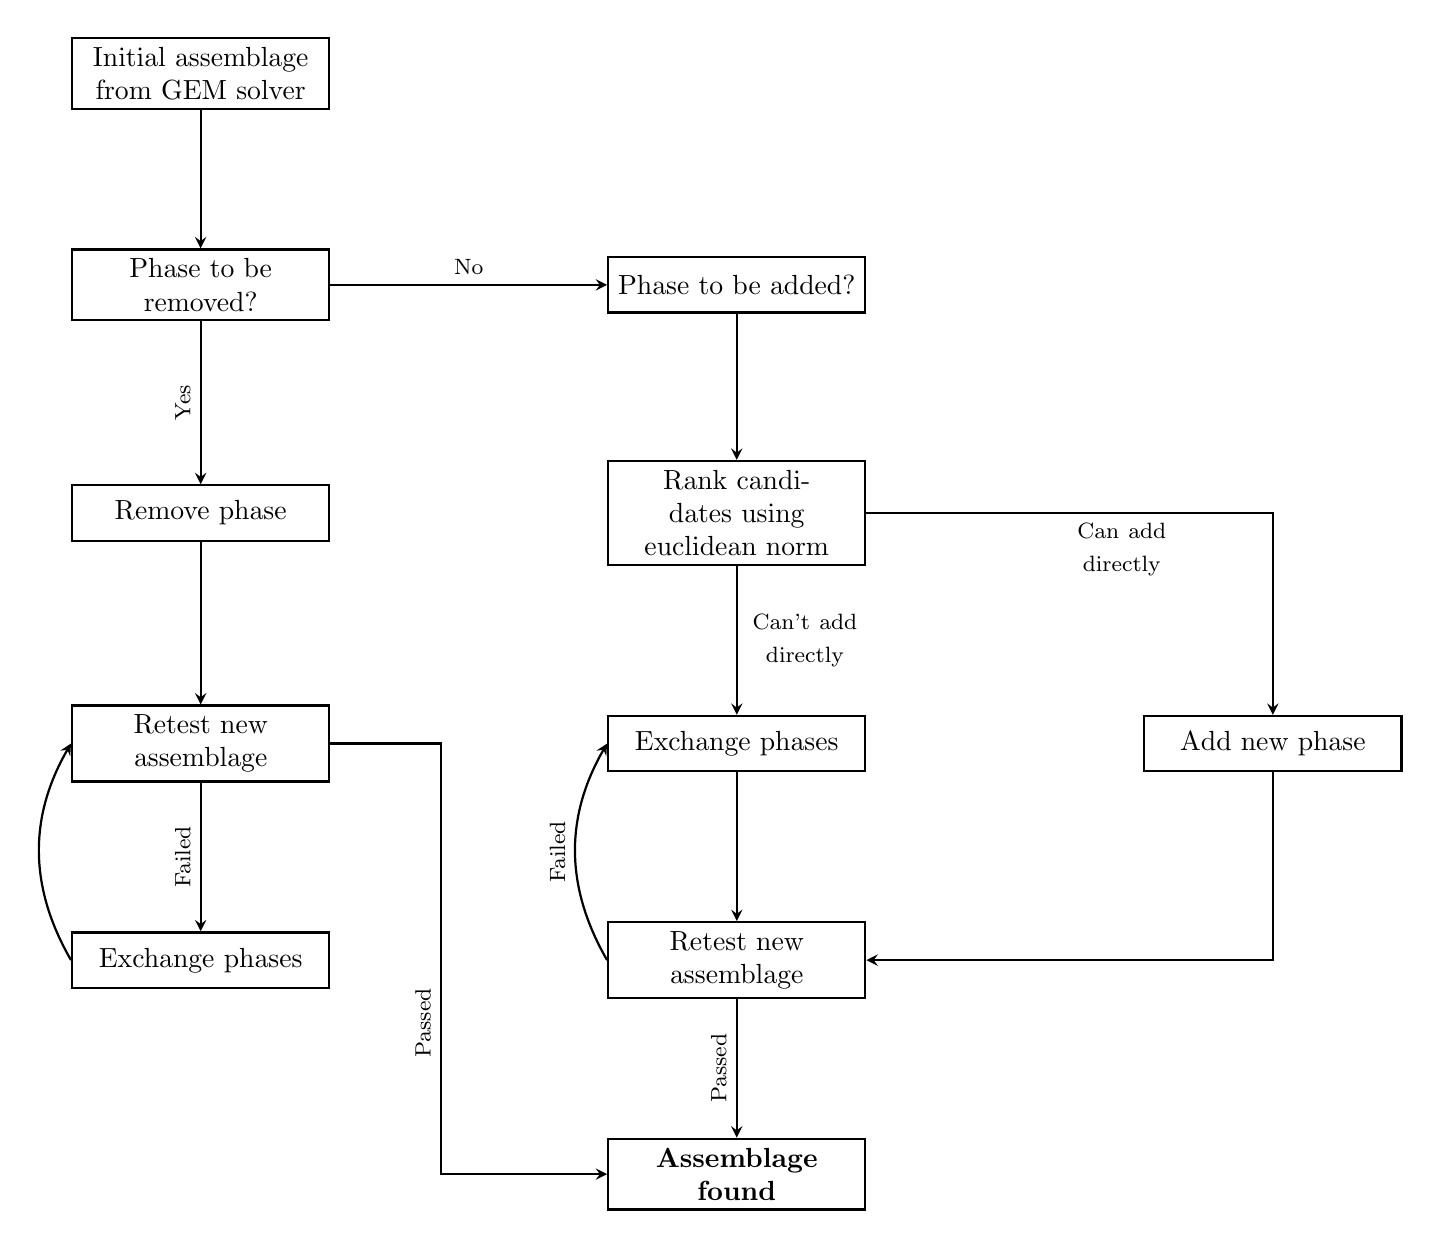
\begin{tikzpicture}[auto,
    			block_center/.style ={rectangle, draw=black, thick, fill=white, text width=0.25\textwidth, text centered, minimum height=2em},
    			block_side/.style ={rectangle, draw=black, thick, fill=white, text width=0.15\textwidth, text centered, minimum height=2em},
			block_noborder/.style ={rectangle, draw=none, thick, fill=none, text width=0.15\textwidth, text centered, minimum height=0.5em},
			block_small/.style ={rectangle, draw=none, thick, fill=none, text width=0.1\textwidth, text centered, minimum height=0.5em},
			line/.style ={draw, thick, -stealth}]
    			% Outlining the flowchart using the PGF/TikZ matrix funtion
    			\matrix [column sep=10em,row sep=5em] {
      				\node [block_center] (00) {Initial assemblage from GEM solver}; & {} \\
      				\node [block_center] (10) {Phase to be removed?}; & \node [block_center] (11) {Phase to be added?}; \\
				\node [block_center] (20) {Remove phase}; & \node [block_center] (21) {Rank candidates using euclidean norm}; & {}\\
				\node [block_center] (30) {Retest new assemblage}; & \node [block_center] (31) {Exchange phases}; & \node [block_center] (32) {Add new phase};\\
				\node [block_center] (40) {Exchange phases}; & \node [block_center] (41) {Retest new assemblage}; & {} \\
				{} & \node [block_center] (51) {\textbf{Assemblage found}}; & {}\\
    			};	% end matrix
    			% connecting nodes with paths
    			\begin{scope}[every path/.style=line]
      				\path (00) edge (10);
     				\path (10) edge node[block_noborder,rotate=90,anchor=south]{\footnotesize{Yes}} (20);
				\path (10) edge node[block_noborder]{\footnotesize{No}} (11);
				\path (20) edge (30);
				\path (30) edge node[block_noborder,rotate=90,anchor=south]{\footnotesize{Failed}} (40);
%				\path (30.360)[-] edge node[block_noborder]{\footnotesize{Passed}} (51.180);
				\path (30.360) -- +(4em,0) |- node[block_noborder,rotate=90,anchor=south west,xshift=2.5em]{\footnotesize{Passed}} (51.180);
				\path[-] (40.180) edge[bend left] (30.180);
				\path (11) edge (21);
				\path (21) edge node[block_noborder,anchor=west,xshift=-0.5em]{\footnotesize{Can't add directly}} (31);
				\path (21.360) -| node[block_noborder,anchor=north east,xshift=-2.5em]{\footnotesize{Can add directly}} (32.90);
				\path (31) edge (41);
				\path (32.270) |- (41.360);
				\path[-] (41.180) edge[bend left] node[block_noborder,rotate=90,anchor=south]{\footnotesize{Failed}}(31.180);
				\path (41) edge node[block_noborder,rotate=90,anchor=south]{\footnotesize{Passed}}(51);
			\end{scope}
 		\end{tikzpicture}
  		\caption{Illustration of the proposed methodology for updating the phase assemblage. Adapted from Piro \cite{Piro17}.}
  		\label{fig:assemblage}
	\end{figure}

\end{landscape}
\restoregeometry

\newgeometry{margin=1cm}
\begin{landscape}
\thispagestyle{empty}

	\begin{figure}
		\centering
		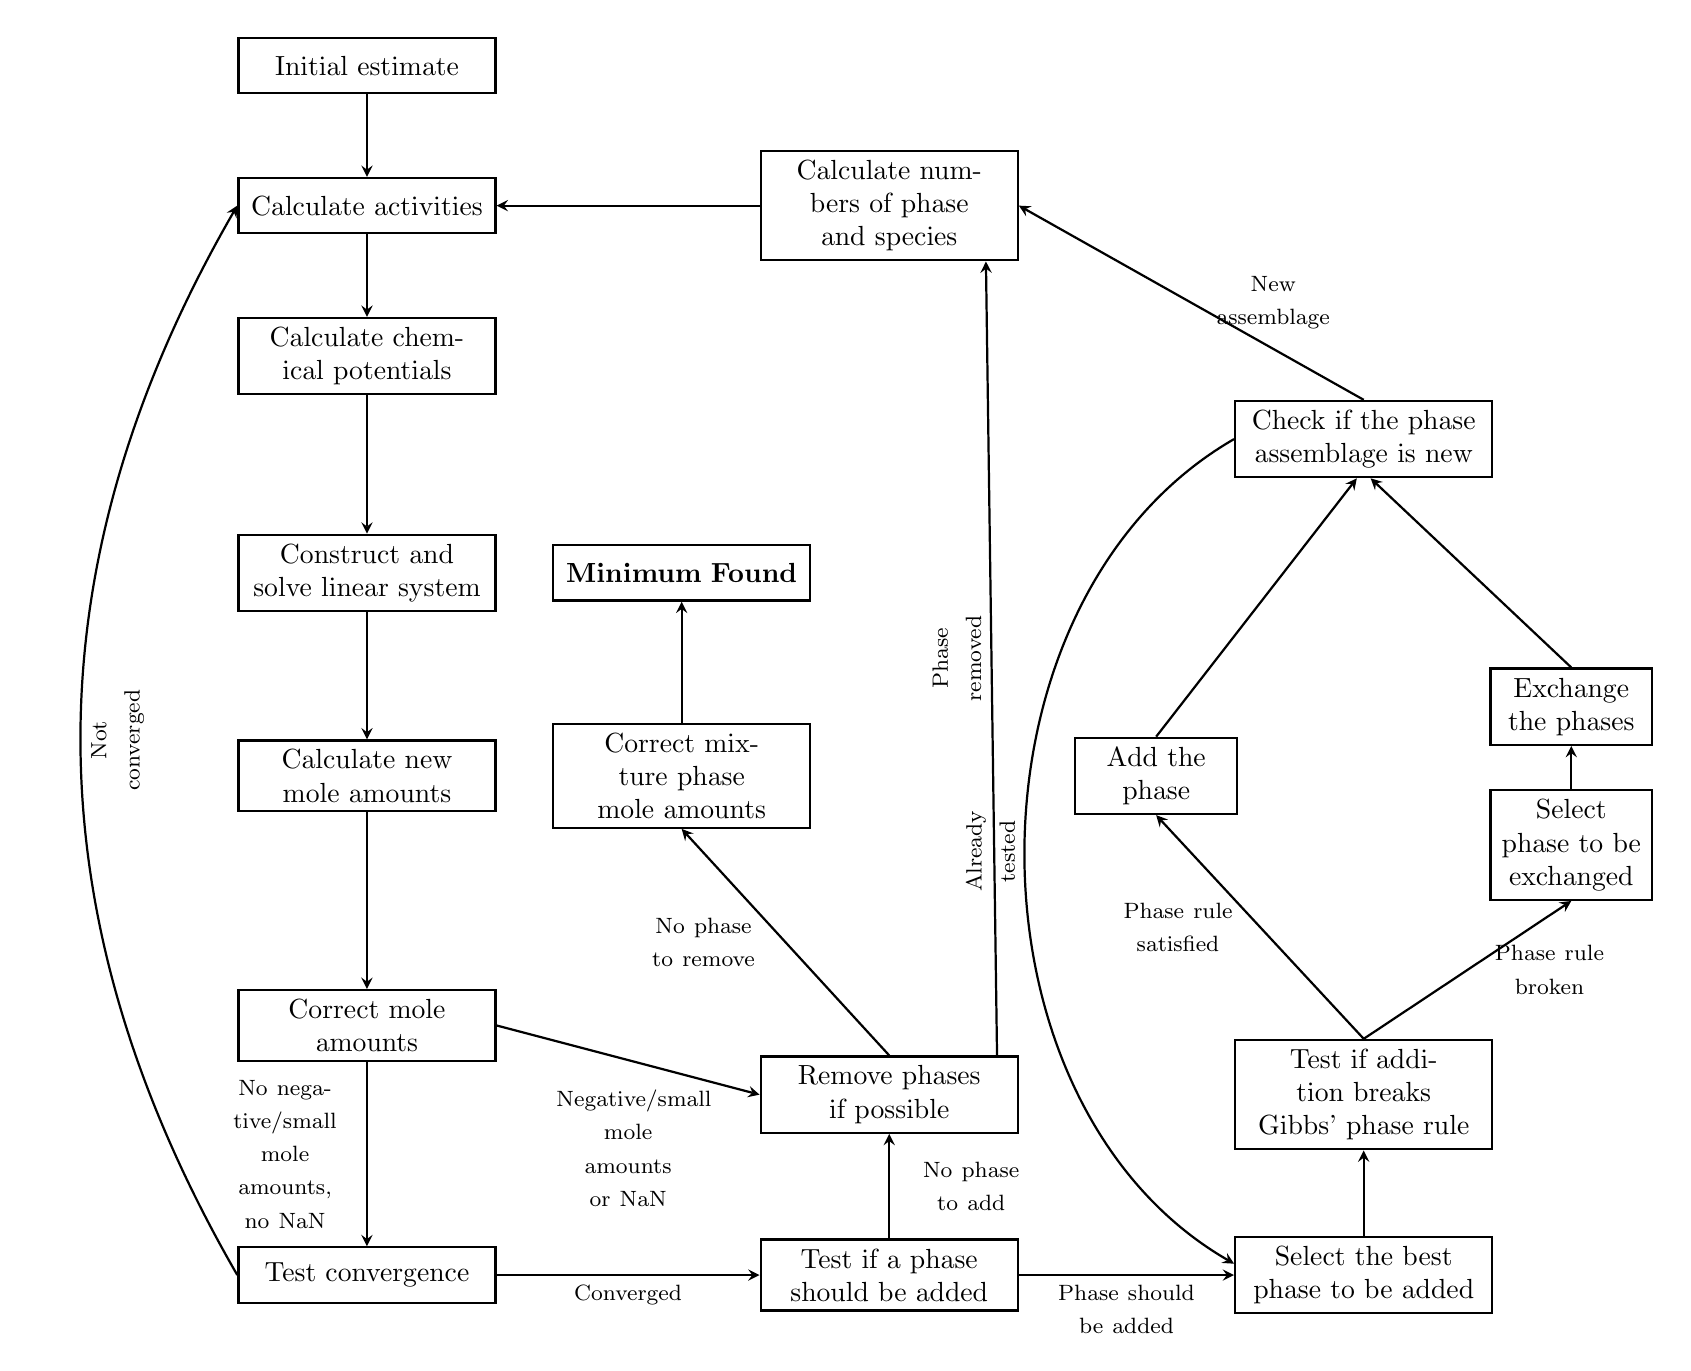
\begin{tikzpicture}[auto,
    			block_center/.style ={rectangle, draw=black, thick, fill=white, text width=0.25\textwidth, text centered, minimum height=2em},
    			block_side/.style ={rectangle, draw=black, thick, fill=white, text width=0.15\textwidth, text centered, minimum height=2em},
			block_noborder/.style ={rectangle, draw=none, thick, fill=none, text width=0.15\textwidth, text centered, minimum height=0.5em},
			block_small/.style ={rectangle, draw=none, thick, fill=none, text width=0.1\textwidth, text centered, minimum height=0.5em},
			line/.style ={draw, thick, -stealth}]
    			% Outlining the flowchart using the PGF/TikZ matrix funtion
    			\matrix [column sep=2em,row sep=2em] {
      				\node [block_center] (00) {Initial estimate}; & {} & {} \\
      				\node [block_center] (10) {Calculate activities}; & \node [block_center] (11) {Calculate numbers of phase and species}; & {}\\
				\node [block_center] (20) {Calculate chemical potentials}; & {} & \node [block_center,yshift=-3em] (22) {Check if the phase assemblage is new};\\
				\node [block_center] (30) {Construct and solve linear system}; & \node [block_center,xshift=-7.5em] (31) {\textbf{Minimum Found}}; & {}\\
				\node [block_center] (40) {Calculate new mole amounts}; & \node [block_center,xshift=-7.5em] (41) {Correct mixture phase mole amounts}; & \node [block_side,xshift=-7.5em] (42a) {Add the phase};  \node [block_side,xshift=7.5em,yshift=-2.5em] (42b) {Select phase to be exchanged}; \node [block_side,xshift=7.5em,yshift=2.5em] (42c) {Exchange the phases};\\
				\node [block_center,yshift=-2.5em] (50) {Correct mole amounts}; & \node [block_center,yshift=-5em] (51) {Remove phases if possible}; & \node [block_center,yshift=-5em] (52) {Test if addition breaks Gibbs' phase rule};\\
				\node [block_center,yshift=-2.5em] (60) {Test convergence}; &  \node [block_center,yshift=-2.5em] (61) {Test if a phase should be added}; & \node [block_center,yshift=-2.5em] (62) {Select the best phase to be added};\\
    			};	% end matrix
    			% connecting nodes with paths
    			\begin{scope}[every path/.style=line]
      				\path (00) edge (10);
     				\path (10) edge (20);
				\path (20) edge (30);
				\path (30) edge (40);
				\path (40) edge (50);
				\path (50) edge node[block_noborder,anchor=east]{\footnotesize{No negative/small mole amounts, no NaN}} (60);
				\path (60) edge node[block_noborder,anchor=north]{\footnotesize{Converged}} (61);
				\path (61) edge node[block_noborder,anchor=north]{\footnotesize{Phase should be added}} (62);
				\path (62) edge (52);
				\path (61) edge node[block_noborder,anchor=west]{\footnotesize{No phase to add}} (51);
				\path[-] (51.90) edge node[block_noborder,anchor=east]{\footnotesize{No phase to remove}} (41.270);
				\path (41) edge  (31);
				\path[-] (51.20) edge node[block_noborder,anchor=south,rotate=90]{\footnotesize{Phase  removed}}(11.330);
				\path[-] (60.180) edge[bend left] node[block_noborder,anchor=north,rotate=90]{\footnotesize{Not converged}} (10.180);
				\path[-] (50.360) edge node[block_noborder,anchor=north,yshift=-0.25cm]{\footnotesize{Negative/small mole amounts or NaN}} (51.180);
				\path[-] (52.90) edge node[block_noborder,anchor=east]{\footnotesize{Phase rule satisfied}}(42a.270);
				\path[-] (52.90) edge node[block_noborder,anchor=west]{\footnotesize{Phase rule broken}}(42b.270);
				\path (42b) edge  (42c);
				\path[-] (42c.90) edge  (22.280);
				\path[-] (42a.90) edge  (22.260);
				\path[-] (22.90) edge node[block_noborder,anchor=west]{\footnotesize{New assemblage}}(11.360);
				\path (11) edge  (10);
				\path[-] (22.180) edge[bend right=60] node[block_noborder,anchor=south,rotate=90]{\footnotesize{Already tested}} (62.175);
			\end{scope}
 		\end{tikzpicture}
  		\caption{Illustration of the proposed Gibbs energy minimisation algorithm. Adapted from Loukusa \cite{Loukusa:2014aa}.}
  		\label{fig:gem_illus}
	\end{figure}

\end{landscape}
\restoregeometry

\section{Global Optimisation}
	The computation of thermodynamic equilibrium, as discussed in sec.~\ref{sec:opt_theory}, is a global optimisation problem where the focus is on systems that can attain equilibrium state under conditions of constant temperature and pressure, where the global minimum value of the Gibbs energy describes the true equilibrium state. The problem can be stated as follows \cite{Floudas99}:
	\begin{objective}
	Given $C$ components participating in up to $\Phi$ potential phases under isothermal and isobaric conditions find the mole vector $\mathbf{n}$ that minimises the value of the Gibbs energy while also satisfying the appropriate material balance constraints.
	\end{objective}

	\begin{constraint}
		The mole fraction of a species in phase $\lambda$, $x_{i(\lambda)}$, must satisfy the following linear equality and inequality constraints
		\begin{equation}
		\sum_{i=1}^{N_\lambda} x_{i(\lambda)} = 1 \mspace{30mu}x_{i(\lambda)} > 0\mspace{30mu} \forall i
		\end{equation}
	\end{constraint}

The component set is represented by the index set $C = \{i\}$ and the elements that constitute these components are given by $E  = \{e\}$. The set of phases is denoted by $\Phi = \{k\}$ where it is composed of solution and stoichiometric phases, labelled $\Lambda$ and $\Omega$ respectively, so that $\Phi \equiv \Lambda\cup \Omega$.

	The conditions for thermodynamic equilibrium discussed in section~\ref{sec:eqb_theory} require that the chemical potentials of all the species must lie on or above the Gibbs plane, which passes through the element potentials $\Gamma_j$. Thus metastable phases must lie above the Gibbs plane and the difference between the Gibbs plane and the plane tangent to a metastable phase is referred to as the \emph{driving force} \cite{Lukas07} or \emph{tangent plane distance function} \cite{Lukas07,Zhang11}. The driving force for solution phase $\lambda$ is represented by $\pi_\lambda$ and is computed as \cite{Piro16}:
	\begin{equation}\label{eq:drivingforce}
		\pi_\lambda = \min_x \sum_{i=1}^{N_\lambda} \left(\mu_{i(\lambda)} - \sum_{j=1}^{C} \nu_{i,j}\Gamma_j \right)
	\end{equation}
	which is subject to the mass balance constraints. The sufficient condition for equilibrium requires that the driving force $\pi_\lambda$ computed with equation~\eqref{eq:drivingforce} is positive for all phases believed to be metastable and zero for all the stable phases. According to Hillert \cite{Hillert81}, the driving force of metastable phases can be evaluated at each iteration to determine whether or not it should be added into the system. However, this function can be non-convex and requires the evaluation of a global minimum and forms the basis of the methods discussed below.

	This section describes three global optimisation methods that have been shown to be promising in thermodynamic  equilibrium calculations. These methods are both stochastic - \emph{particle swarm optimisation} and deterministic - \emph{grid construction} and \emph{branch and bound}.

	\subsection{Particle Swarm Optimisation}
	Particle Swarm Optimisation (PSO) has been inspired by the swarm like behaviour in the animal kingdom such the migration of swarm of bees \cite{Kennedy95}. In this method, a population of candidate solutions, dubbed particles, moves around the search space as function of the position and velocity of the particle. the movement of each particle is influenced by it's best known local position and guided towards the best global position as other particles find better solutions.

	The position vector of the particles at iteration $m$, $\mathbf{x_p^m}$, is updated based on the velocity vector, $\mathbf{v_p^m}$, by \cite{Piro16}:
	\begin{gather}
		\mathbf{v_p^m} = \psi \mathbf{v_p^{m-1}} + \phi_p r_p \left(\mathbf{x_p^*} - \mathbf{x_p^m}\right) + \phi_s r_s \left(\mathbf{x_s^*} - \mathbf{x_p^m}\right) \label{eq:PSO1}\\
		\mathbf{x_p^{m+1}} = \mathbf{x_p^m} + \mathbf{v_p^m} \label{eq:PSO2}
	\end{gather}
	where, $x_p^*$ denotes the best known position of a particle (local minima) and $x_s^*$ denotes the best known position of the swarm (global maximum). The first term in the above equation can be interpreted as the inertia term while the second and the third terms act as the driving force towards the local minima and global minimum respectively. These terms are weighted by the parameters $\psi$, $\phi_p$ and $\psi_s$ which can be tuned according to the problem. These parameters affect the behaviour and efficacy of the PSO algorithm. Finally, randomly generated numbers $r_p, \; r_s \in (0,1)$ influence the movement of the swarm towards the local or global optima.

	The implementation of PSO is an iterative process where $N_\lambda$ are initially released at $N_\lambda$ corners in domain and and allowed to traverse the domain with the velocity and position being updated through \eqref{eq:PSO1} and \eqref{eq:PSO2} respectively. At each iteration, the velocity vector must also be scaled to ensure that the particle stays within the feasible region, i.e, $0 < x_{i(\lambda)}<1$ \cite{Piro16}.

	A challenge in the implementation of the PSO algorithm will be to tune the parameters $\psi$, $\phi_p$ and $\psi_s$ to achieve a compromise between good convergence rate and thoroughness in traversing the search space. Piro and Simunovic \cite{Piro16} have found that $\psi=0.5$, $\phi_p=2$ and $\psi_s=2$ provides the desired behaviour and that the parameters can be tuned effectively by progressively relaxing the constraints imposed on the velocity magnitude using the following equation \cite{Nocedal06}:
	\begin{equation}\label{eq:PSOvel}
		\|\mathbf{v}\| \leq v_{min} + \frac{v_{max}-v_{min}}{m_{max} - 1} (m-1)
	\end{equation}
	where, $v_{max}$ and $v_{min}$ are the pre-specified maximum and minimum velocity magnitudes respectively and $m_{max}$ is the maximum number of iteration allowed in PSO. Thereby, the optimisation neighbourhood gradually increases in size as the iteration cycle progresses.

	\subsection{Grid Construction}
	Grid construction has been widely adopted in thermodynamic equilibrium codes as a strategy for testing equilibria by performing numerous evaluations of the objective function at regular intervals in the domain \cite{Shobu09,Sundman85,Sundman15,Chen93a,Chen93b}. The method was developed in the 1970s and 1980s as a brute force method to verify global minimum for phase diagram construction problems and does not scale well for large systems. As shown in figure~\ref{fig:Grid_cons}, in the grid construction method, the surface of $\pi_\lambda$ is discretised with each point treated as a stoichiometric compound and the ensemble of these compounds collectively approximates the driving force surface \cite{Piro16}. In the example figure, the arbitrary binary system consists of a solution phase and a stoichiometric phase and the domain for the solution phase has been divided into 11 grid points.
	\begin{figure}[htbp]
		\centering
		\includegraphics[width=0.65\textwidth]{figures/Grid_const}
		\caption{Demonstration of the grid construction method for an arbitrary binary system at constant temperature and pressure. The domain has been discretised into 11 grid points and the pure stoichiometric phase \ce{A3B2} is found to be in equilibrium with the solution phase giving a false positive \cite{Piro16}.}
		\label{fig:Grid_cons}
	\end{figure}

The discretisation of the grid plays an important role in the efficacy of this method and it has been shown by Chen \textit{et al.} \cite{Chen93b} that the grid must be sufficiently resolved to avoid missing critical features such as the minimum between $\alpha_1$ and $\alpha_2$ in  fig.~\ref{fig:Grid_cons}.  However, this requirement leads to commercial concerns as too small a grid leads to an increase in the computational cost while too large a grid can lead to false positives in the optimisation process.  Piro and Simunovic \cite{Piro16} have demonstrated how uniformly spaced grid for a solution phase $\lambda$ in $N_\lambda$ dimensional Euclidean phase (each dimension corresponds to a species in phase $\lambda$) can result in an enormously large number of grid points depending on the grid size. While Chen \textit{et al.} \cite{Chen93a} and the open-source code \texttt{OpenCalphad} \cite{Sundman:2015aa} use 8 grid points, it becomes clear from figure~\ref{fig:Grid_cons} that global minimum would not be found. Therefore, the rapid increase in the computational cost with the reduction in grid size and a questionable performance in terms of reaching a global maximum tilts the scales against this method.

	\subsection{Branch and Bound}
	The Branch and Bound (B\&B) algorithm was proposed to solve constrained optimisation problems for non-convex functions by solving a sequence of problems in each of which the objective function is convex \cite{Falk69}. The algorithm involves two procedures to solve global optimisation problems:
	\begin{enumerate}
		\item \textbf{Branching}: The domain $D$ is partitioned into two or more smaller disjoint domains $D_1,D_2,\dots,$ such that $D = D_1 \cup D_2 \cup \dots$ Thus, the partitioned objective function can be considered a convex approximation of the objective function within the subdomain $D_i$.
		\item \textbf{Bounding}: The upper and lower bound of the objective function are found within a subset of the domain $D$. In the classical Branch and Bound method, a subdomain can be removed from the analysis the lower bound of the objective function in it is greater than the upper bound of the objective function in any other subdomain.
	\end{enumerate}

	 While the B\&B method was originally applied to mixed integer linear programming (MINLP) problems \cite{Jaulin01}, McDonald and Floudas \cite{McDonald95} applied it to solve thermochemical equilibrium problems. Piro and Simunovic \cite{Piro16} proposed a modified version of the classical B\&B for \texttt{Thermochimica} which uses a different initialisation procedure and relaxation scheme for the bounds. Furthermore, instead of relying on pruning, every subdomain is evaluated till stopping criteria are met and if necessary, recursive partitioning technique is applied.

	 The approach adopted by Piro and Simunovic \cite{Piro16} partitions the domain for each solution phase $\lambda$ into $N_\lambda$ subdomains and the driving force $\pi_\lambda$ is minimised in each subdomain. The Lagrangian function of the driving force of the solution phase $\lambda$ can be defined as follows \cite{Piro16}:
	 \begin{equation}
	 	L_\lambda = \sum_{i=1}^{N_\lambda} x_{i(\lambda)}\left( \mu_{i(\lambda)} - \sum_{j=1}^{C} \nu_{i,j}\Gamma_j \right) - \pi_{\lambda}\left( \sum_{i=1}^{N_\lambda} x_{i(\lambda)} -  1 \right)
	 \end{equation}
	 In the branch and bound method, the local variables (mole fraction of species, $x_{i(\lambda)}$, and driving force $\pi_{\lambda}$) are optimised while holding the global variables (element potentials i.e. $\Gamma_j$) constant. This results in a system of $N_{\lambda} + 1$ equations for a particular phase $\lambda$. To find the minimum, differentiating $L_\lambda$ with respect to $x_{i(\lambda)}$ and $\pi_{\lambda}$ and applying the Gibbs-Duhem equation:
	 \begin{gather}
	 	\frac{\partial L_\lambda}{\partial x_{i(\lambda)}} = \mu_{i(\lambda)} - \sum_{j=1}^{C} \nu_{i,j}\Gamma_j + 1 - \pi_{\lambda} \\
		\frac{\partial L_\lambda}{\partial \pi_{\lambda}} = 1- \sum_{i=1}^{N_\lambda} x_{i(\lambda)}
	 \end{gather}

	 Taking a second order Taylor approximation of the Lagrangian function,
	 \begin{equation}
	 	\nabla^2 L_\lambda \delta y =  - \nabla L_\lambda
	 \end{equation}
	 where the column vector of unknown variables $\delta y = [\delta x, \delta \pi]^T$. The second order partial derivatives are equal to:
	  \begin{gather}
	 	\frac{\partial^2 L_\lambda}{\partial x_{i(\lambda)}^2} = \frac{1}{x_{i(\lambda)}} \mspace{50mu} \frac{\partial^2 L_\lambda}{\partial x_{i(\lambda)} \partial x_{j(\lambda)}} = 0 \\
		\frac{\partial^2 L_\lambda}{\partial \pi_{\lambda} \partial x_{i(\lambda)}} = 0 \mspace{50mu}  \frac{\partial^2 L_\lambda}{\partial \pi_{\lambda}^2} = 0
	 \end{gather}

	 The discussion can be extended to incorporate charge neutrality constraints through the following equation:
	 \begin{equation}
		L_\lambda = \sum_{i=1}^{N_\lambda} x_{i(\lambda)}\left( \mu_{i(\lambda)} - \sum_{j=1}^{C} \nu_{i,j}\Gamma_j \right) - \pi_{\lambda}\left( \sum_{i=1}^{N_\lambda} x_{i(\lambda)} -  1 \right) - \pi_e \left( \sum_{i=1}^{N_\lambda} \nu_{i,e} x_{i(\lambda)} -  1\right)
	\end{equation}
	where $\pi_e$ denotes the Lagrange multiplier of the electronic component.

	Solving the first order partial differential gives:
	\begin{equation}
	\frac{\partial L_\lambda}{\partial \pi_e} = 1 - \sum_{i=1}^{N_\lambda} \nu_{i,e} x_{i(\lambda)}
	\end{equation}

	The second order terms are the following:
	\begin{equation}
	\frac{\partial^2 L_\lambda}{\partial \pi_e^2} = 0 \mspace{50mu} \frac{\partial^2 L_\lambda}{\partial \pi_e \partial x_i} = -\nu_{i,e}
	\end{equation}


	 The Hessian in the above system of equations can be represented as a symmetric arrow matrix:
	 \begin{equation}\label{eq:BB_mat}
        		\mathbf{H} =
        		\begin{bmatrix}
            		\frac{1}{x_{1(\lambda)}} & {} & {} & {} & -1 \\
		 	{} & \frac{1}{x_{1(\lambda)}} & {} & {} & -1 \\
			{} & {} & {\ddots} & {} & \vdots \\
			{} & {} & {} & \frac{1}{x_{N(\lambda)}} & -1 \\
			{-1} & {-1} & {\dots} & {-1} & 0
        		\end{bmatrix}
   	\end{equation}

	Therefore, by exploiting the structure of this matrix, the combination of ${x_{i(\lambda)}}$ that minimises ${\pi_{\lambda}}$ can be easily determined. To solve the above matrix, Gaussian elimination can be performed on the just the bottom row followed by back substitution. Furthermore, instead of storing a Hessian, the diagonal vector and a scalar representing the far right column can be stored. However, the implementation of this method warrants the use of an appropriate line search algorithm to ensure that the Wolfe conditions are satisfied and that the local system stays within the feasible region $0 < x_{i(\lambda)}<1$ . In addition, the step length must be suitably constrained to avoid missing any local minimums \cite{Piro16}.

	The application of the branch and bound method to the arbitrary binary problem presented before has been illustrated in figure~\ref{fig:BB_1}. Piro and Simunovic implemented an iterative technique where the domain was initially divided into 2 subdomains with the initialisation of each sub-domain at the corners. To improve numerical stability, the bounds of each subdomain were relaxed while the domain bounds were strictly enforced. The stopping criteria within a subdomain was convergence to local minimum or departure of the local minimiser from the subdomain. In case multiple minima were encountered within a subdomain, the subdomain was further split at the next iteration.

	\begin{figure}[htbp]
		\centering
		\includegraphics[width=0.65\textwidth]{figures/BB1}
		\caption{Demonstration of the branch and bound method for an arbitrary binary system at constant temperature and pressure. The domain has been partitioned into 2 subdomains \cite{Piro16}.}
		\label{fig:BB_1}
	\end{figure}

	The branch and bound method was able to identify the local minima in both the domains and subsequently the predicted phase assemblage was found to be at the global minimum as shown in figure~\ref{fig:BB_2}

		 \begin{figure}[htbp]
		\centering
		\includegraphics[width=0.65\textwidth]{figures/BB2}
		\caption{Refinement of the subdomains in branch and bound method and the subsequent convergence to global minimum \cite{Piro16}.}
		\label{fig:BB_2}
	\end{figure}

	  All global optimisation methods have their advantages and disadvantages and no global optimisation method is universally superior to others. While the deterministic methods are good at converging to a local minimum, they are often prone to high computational expenses. The stochastic methods, on the other hand, tend to cover the search space more effectively but face difficulty at finding the global minimum \cite{Piro16}. The global optimisation methods discussed in literature have mostly been problem centric and there has been a lack of a comprehensive and rigorous analysis of these methods applied to a variety of thermodynamic equilibrium problems. Therefore, apart from the non-linear solver, this work will also focus on a quantitative comparison of global optimisation methods in terms of application to thermodynamic equilibrium calculations. This comparison will be based on evaluating the reliability, capability and performance of the methods and some preliminary details of the methodology will be discussed in section~\ref{sec:workplan}


\section{Integration in multiphysics codes}
	The thermodynamic solver is being developed with the primary aim of being incorporated within the  finite element multiphysics framework \texttt{MOOSE}. The first level of integration of the thermodynamic solver within \texttt{Yellowjacket} will be coupling thermodynamic equilibrium calculations with kinetics and phase field modules being developed by at the Idaho National Laboratory and the University of Florida. This would involve procedures to transfer information between the thermodynamic solver and the other modules. Though  \texttt{MOOSE} contains the tools required to enable such computations with minimum effort, there always remains a probability of conflicts arising during coupling, such as conflicting variables, etc. Also, different \texttt{MOOSE} apps have different requirements from the thermodynamic equilibrium solver. While \texttt{Marmot} and \texttt{Bison} computations are mostly require partial derivatives of Gibbs energies (chemical potential, driving force, etc.) and assemblages, other codes might require quantities such as the heat capacity, thermal conductivity, etc.  Therefore, though the procedures have not yet been finalised, complete integration of the thermodynamic solver in \texttt{MOOSE} will be a major focus towards the end of this project.



\section{Summary}
	A number of algorithms for different parts of a thermodynamic equilibrium solver were presented in this chapter. Many of these algorithms have already been implemented in other codes available in the literature and GEM and levelling are relatively mature algorithms with little to no scope of improvement. This is evident from the fact that most of the development efforts since the original GEm method has relied on auxiliary operations such as initialisation, etc. However, this does not mean that improvements can not be made.  The development of an advanced thermodynamic solver leaves the door open for incremental gains on many of these algorithms.
For example, the post-levelling and temporal series estimates for initialisation will be more carefully analysed and implemented during this work in order to minimise the computational cost of the non-linear step. The work on non-linear step will focus on improving the convergence rate by focussing the attention on the line-search and phase update algorithms. Finally, two of the major areas that stand to benefit from this work are global optimisation methods and integration with multiphysics framework \texttt{MOOSE}. The rigorous application based study of global optimisation methods which will be performed during this work is expected to provide a definitive answer to the question of reliability, efficiency and robustness of various candidate methods for application to thermodynamic equilibrium problems. The optimum method will then be implemented to achieve the best possible performance. Regarding \texttt{MOOSE} integration, this work will try to minimise the costs associated with thermodynamic equilibrium calculations, which significantly impede performance of multiphysics simulations, by minimising thermodynamic computation costs themselves  and reducing overheads  related to coupling which also contribute towards the performance impediment.
